\subsection{Usar el complemento generador de cuadrículas}

El generador de cuadrículas permite crear una «malla» de puntos, líneas o
polígonos que cubra nuestro área de interés. Se deben introducir todas las
unidades en grados decimales. La salida es un archivo shape que se puede
proyectar al vuelo para ajustarlo a sus otros datos.

\begin{figure}[ht]
\begin{center}
  \caption{Crear una capa de cuadrícula}\label{fig:graticule}\smallskip
  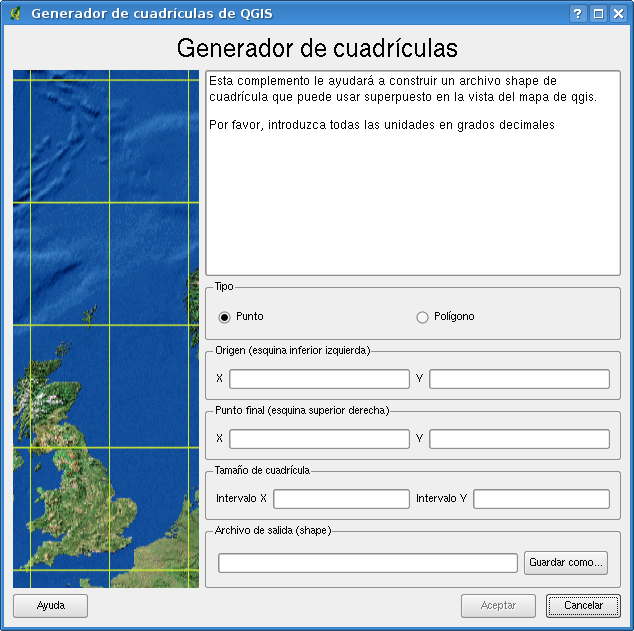
\includegraphics[scale=0.5]{graticule}
\end{center}
\end{figure}

Aquí hay un ejemplo de cómo crear una cuadrícula:

\begin{enumerate}
\item Asegúrese de que el complemento está cargado.
\item Pulse en la herramienta \textsl{Generador de cuadrículas} en la barra de herramientas de complementos.
\item Seleccione el tipo de cuadrícula que quiera crear: punto, línea o polígono.
\item Introduzca la latitud y la longitud para las esquinas inferior izquierda y superior derecha de la cuadrícula.
\item Introduzca el intervalo a usar para construir la cuadrícula. Puede introducir
  valores diferentes para las direcciones X e Y (longitud, latitud).
\item Seleccione el nombre y la localización del archivo shape a crear.
\item Pulse \textsl{Aceptar} para crear la cuadrícula y añadirla a la vista del mapa.
\end{enumerate} 


